\documentclass[a4paper,12pt]{article}
\usepackage[top=2cm,bottom=2cm,left=2cm,right=2cm]{geometry}
\usepackage[utf8]{inputenc}
\usepackage{graphicx}
\usepackage[fontset=macnew]{ctex}
\usepackage{verbatim}
\usepackage{enumitem}
\usepackage{floatrow}
\usepackage{stmaryrd}
\usepackage{amsmath,amsthm,amssymb}
\usepackage{multicol}
\usepackage{wrapfig}
\usepackage{cancel}
\usepackage{subcaption}

\setlist{noitemsep}

\graphicspath{ {./images/} }

\title{Enigma破译\ 实验报告}
\author{陈庆之 2021011819}

\begin{document}
	
	\maketitle
	
	\section{算法原理}
	\subsection{Enigma原理}
	
	本次实验破译的是Enigma I型号,它有三个转子:
	
	\begin{center}
		\begin{tabular}{||c|c|c||}
			\hline 
			序号 & 接线顺序 & 进位格 \\
			\hline 
			I & EKMFLGDQVZNTOWYHXUSPAIBRCJ & R \\
			\hline 
			II & AJDKSIRUXBLHWTMCQGZNPYFVOE & F \\
			\hline 
			III & BDFHJLCPRTXVZNYEIWGAKMUSQO & W \\
			\hline
		\end{tabular}
	\end{center}

	
	\begin{wrapfigure}{r}{0.3\textwidth}
		\centering
		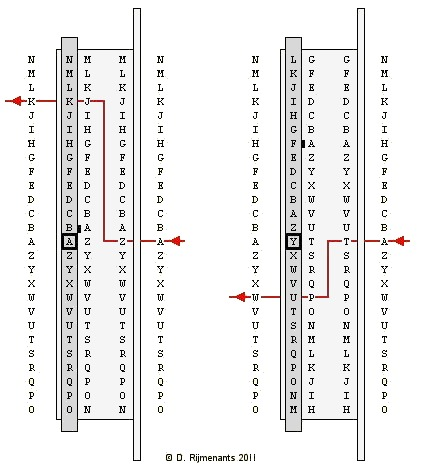
\includegraphics[width=\textwidth]{rotorencodewithring}
	\end{wrapfigure}
	
	
	同时,可以为每个转子指定Ring Setting,这可以使其输入端口和\textit{实际使用的接线端口}之间产生一个轮换映射。若Ring Setting的字母序号为n,则在输入时\textit{视为}输入了输入字母-n的字母,信号会依照这个新字母进入转子的对应接线口;映射完成后,信号会从某个接线口输出,但\textit{视为}输出了输出字母+n的字母。(这和Current Position相互独立;但Current Position的作用机制是类似的。Enigma的密钥本质上是Ring Setting和Initial Position之间的差值,因此\textit{本实验中固定Ring Setting=DES,尝试破解Initial Position.})
		
	右图分别展现了Ring Setting = 'B', Current Position = 'A'和Ring Setting = 'F', Current Position = 'Y'时,转子I在输入信号A时的表现。
	
	每次输入一个信号(一个字母),最右侧的转子就会拨动一格。若这次拨动使得最右侧转子达到了上表中\textbf{进位格}记录的字母,就会带动它左侧的转子(也就是中间转子)前进一格。如果这次前进使得中间转子达到了\textbf{进位格的前一格},那么中间转子会在下一个信号时立刻再前进一格,连带最左侧转子也一同前进一格。这被称为\textbf{Double Stepping},是由于三个转子位置上的机械结构并不完全对称导致的。
	
	Enigma的加/解密具有自反性:解密一段密文的方式就是使用加密时相同设置的Enigma,再”加密“一次密文就可得到明文。
	
	\subsection{Rejewski的方法}
	
	Rejewski的方法利用了当时德国人发报的一个流程,即在密报开头连续书写两次某三个字母在当日密钥加密下的密文,然后使用这三个字母加密余下的明文。虽然这不显式地提供关于每日密钥的信息,但是它泄露了在当日密钥加密下相隔3的两个相同字母密文的对应关系。
	
	设在当日设置的Enigma密码机中,第k位的映射关系为$A_k$,某条消息密钥为$L_iL_jL_k$,该密文的开头六个字母为$L_1\dots L_6$.假设没有插线板交换,那么有$A_1(L_i) = L_1, A_4(L_i) = L_4$.由enigma加密的自反性,有$A_1(L_1) = L_i$,即$A_4(A_1(L_1)) = L_4$.如果我们有大量同一日的密文,就可以获得$L_1$到$L_4$的映射表,这个映射是一个字母表的重排。我们可以从中找到所有的环并记录其长度。对于$L_2$和$L_5$、$L_3$和$L_6$同样可以获得环长序列。由于密钥到环长序列的对应关系是单射,我们可以根据长度序列构建密钥的等价类。根据每天获得的$L_1$到$L_4$的映射表,就可以将密钥空间缩小到所在等价类中。
	
	Lejewski发现,即使我们考虑插线板的交换,也不会影响上述环的长度序列(只是参与环的字母发生了变化)。因此上述方法不依赖于插线板不存在的假设。我们可以遍历所有转子序列和密钥,构建上面所说的等价类并组织成查询表供实际破译使用。对于最后可能出现的多种密文,只需观察是否有接近可读文字的片段就能确认使用的密钥是哪一个(本质上是普通置换密码的破译)。
	
	\subsection{Turing的方法}
	
	Turing的方法是一种已知明文攻击,主要用于攻破德军增加转子数量、增加接线板复杂度之后的安全升级,同时不依赖于德军开头三字母重复的行为。
	
	设明文为$L_1\dots L_n$,密文为$M_1\dots M_n$,当日第k位在无接线板的情况下映射关系为$A_k$,接线板的映射关系为$R$,则$\forall k < n, M_k = RA_kR(L_k)$. Turing观察到,如果存在环$C: E_1\dots E_mE_1\ s.t.\forall i < m, RA_{k_i}R(E_i) = E_{i+1}$,则有$E_1 = RA_{k_n}\cancel{R}\cancel{R}A_{k_{n-1}}\cancel{R}\dots \cancel{R}A_{k_1}R(E_1)$,其中所有相邻的$R$均因自反性被抵消;可以根据$R$的自反性推得$R(E_1) = A_{k_n}A_{k_{n-1}}\dots A_{k_1}R(E_1)$。由于所有的$k_i$均已知,可以通过遍历每一种转子设定以及$R(E_1)$,检查这种转子设定下能否使$R(E_1)$成环即可。如果某个转子设定下不存在这样的$R(E_1)$,那就可以排除这种转子设定。由于德军的电报内容时常有重复,这样的圈可以找到复数个,这就要求筛选时满足所有的成环性质,进一步提升了筛选的效率。更进一步地,如果某种转子设定和$R(E_1)$的组合通过了上述检验,那么我们还能确定接线板上把$E_1$和$R(E_1)$接在了一起(如果$E_1 = R(E_1)$则证明$E_1$没有接线)。
	
	虽然上述检验只是命中密钥的必要条件,但也能将密钥空间以指数级($\frac{1}{26^k}$)的效率缩小。
	
	\section{实际攻击样例}
	
	\subsection{Rejewski的方法}
	\noindent\textbf{条件}:已知前六位的对应关系分别是ELCONWDIAPKSZHFBQTJYRGVXMU, MRWJFDVSQEXUCONHBIPLTGAYZK和WADFRPOLNTVCHMYBJQIGEUSKZX。
	
	\begin{figure}[h]
		\centering
		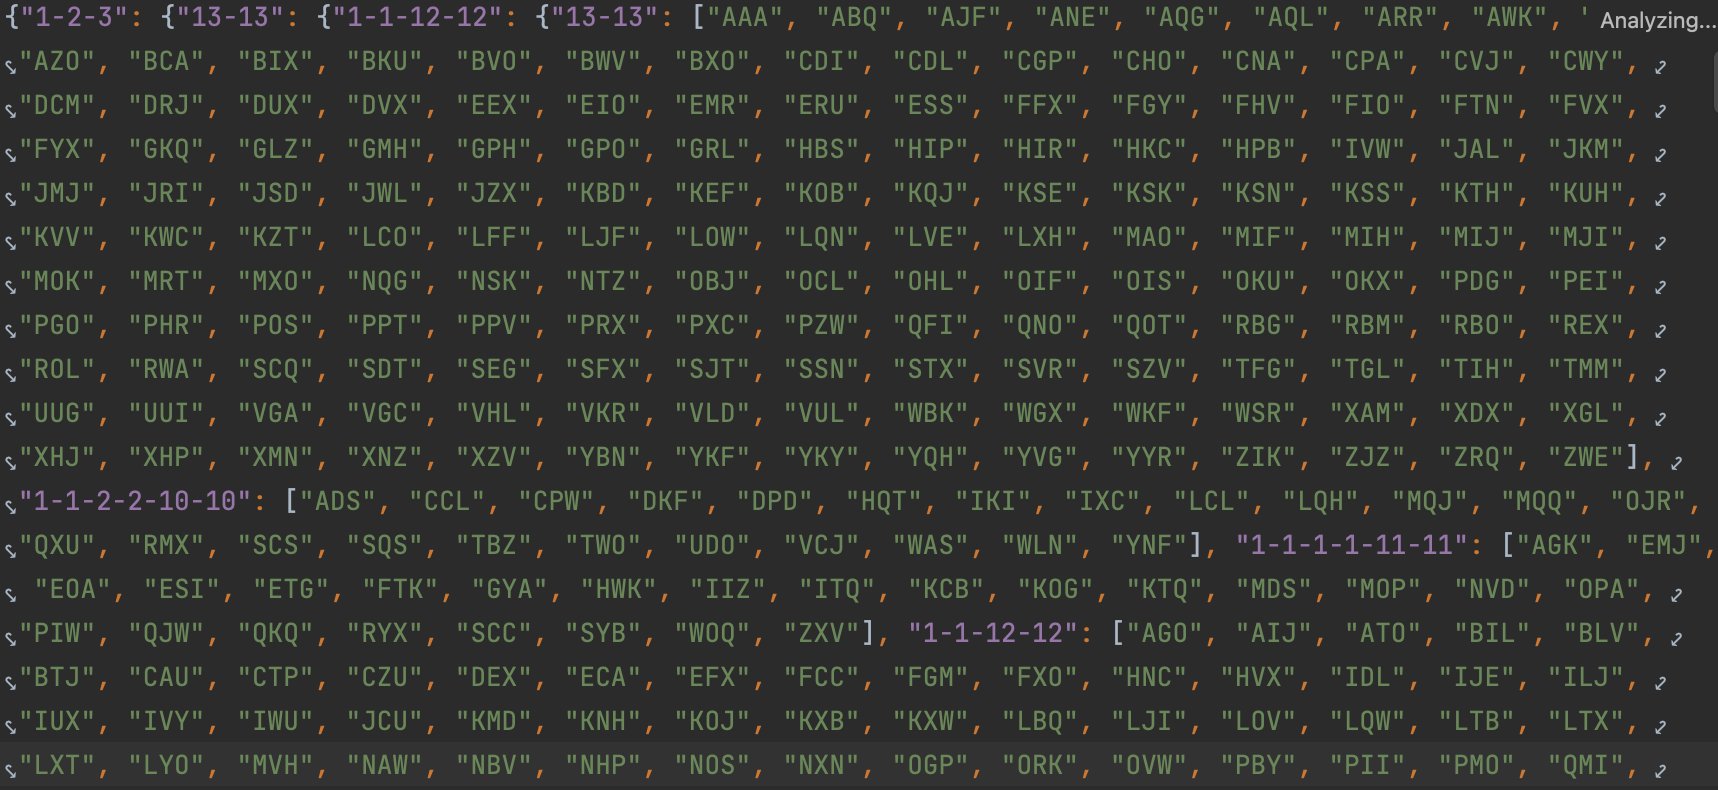
\includegraphics[width=0.9\textwidth]{rejcatalogue}
		\caption{catalogue.json节选}
	\end{figure}

	我们先构建了一个分类库(见上图),约定最外层key为转子顺序,key为环长度序列的升序排列。这个构建过程耗时约45s。之后根据已经制作好的分类库,输入前六个字母的对应关系以及一段密文,代码会给出所有可能的转子顺序、初始位置和明文的对应关系,只需观察哪种情况更接近可读文字即可。
	
	\begin{figure}[h]
		\centering
		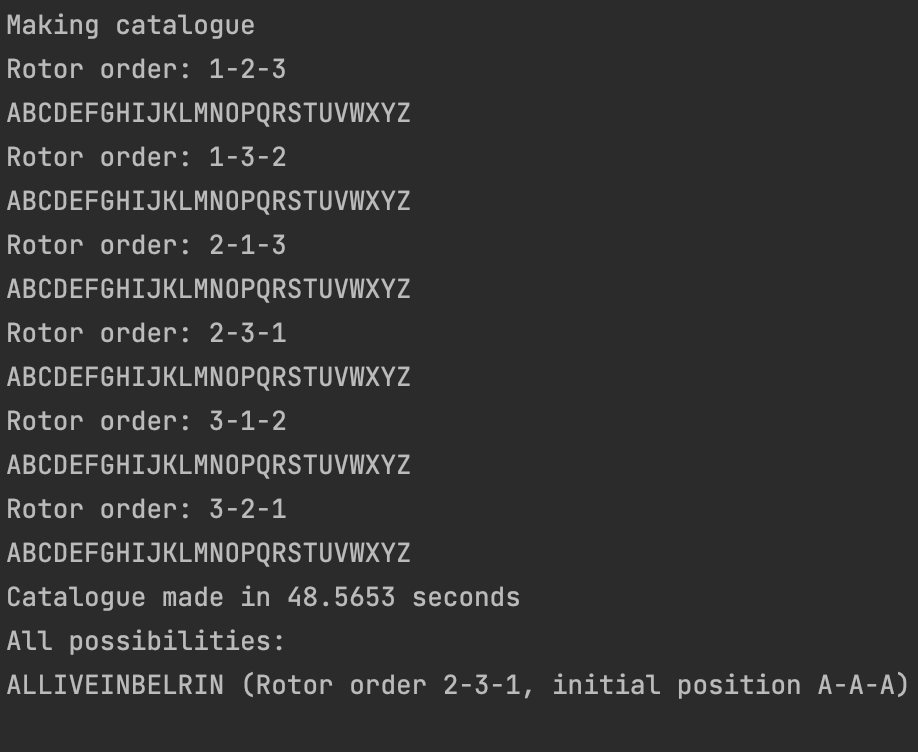
\includegraphics[width=0.5\textwidth]{rej}
		\caption{作业给定enigma的破解过程(含catalogue制作,假定原文为ARRIVEINBERLIN)}
	\end{figure}
	
	
	\subsection{Turing的方法}
	
	\noindent
	\begin{figure}
	\centering
		\begin{subfigure}{.4\textwidth}
			\centering
			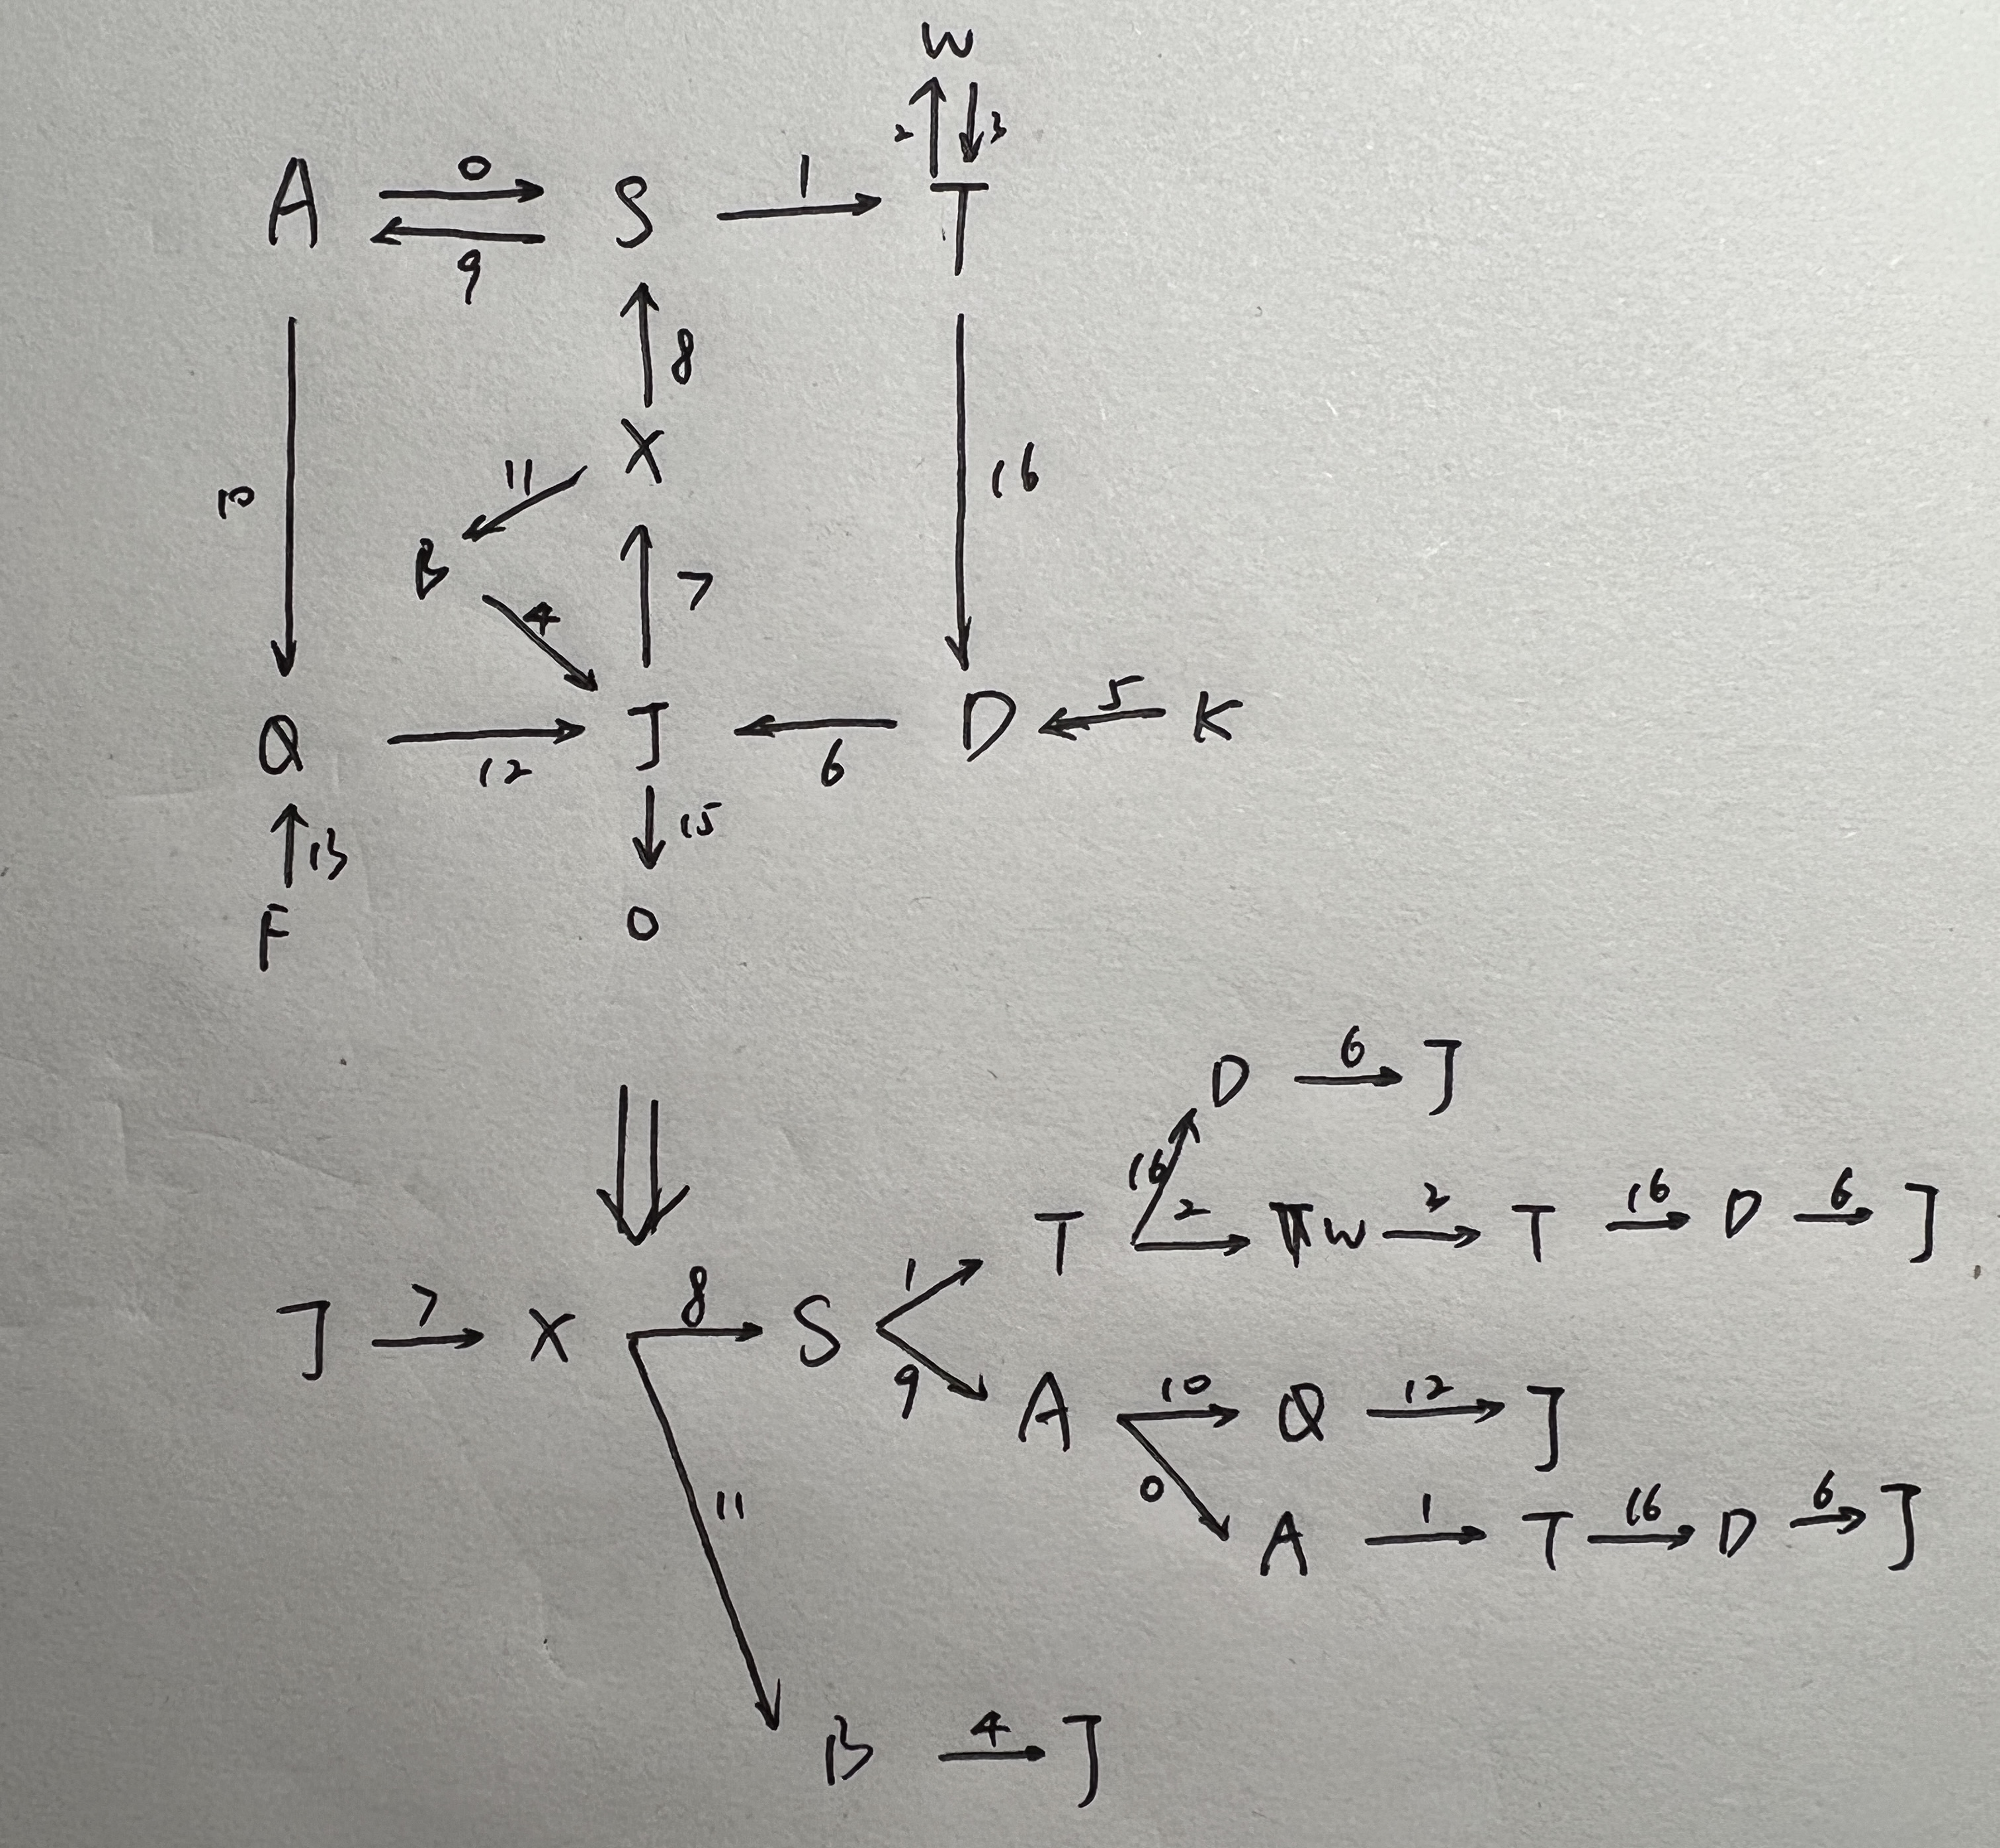
\includegraphics[width=\linewidth]{turingring}
			\caption{作业给定enigma的环图,环路的根为J}
		\end{subfigure}
		\begin{subfigure}{.55\textwidth}
			\centering
			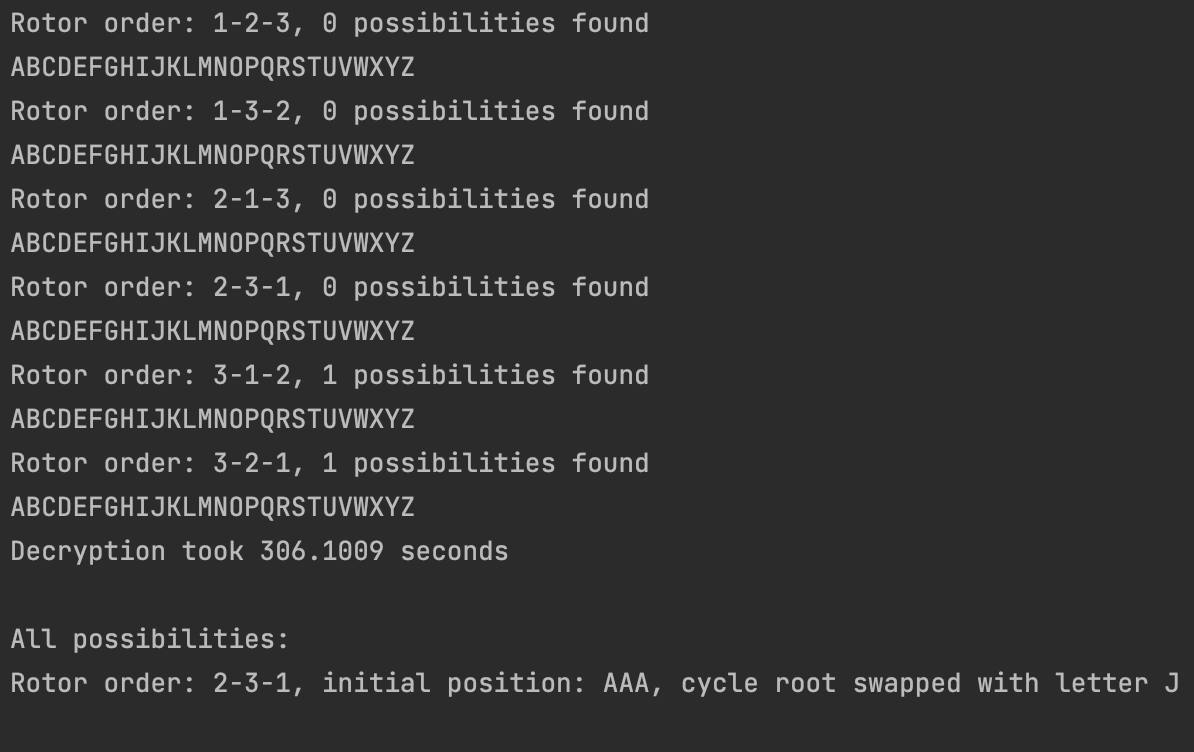
\includegraphics[width=0.9\linewidth]{turing}
			\caption{程序破译结果}
		\end{subfigure}
	\end{figure}

		如上图,输入环路信息,程序开始枚举每一种可能性,最后输出满足所有环路条件的转子顺序、初始位置和对应关系(程序预测J与自身交换,说明J在接线板上没有连线)。
	
	\section{代码结构}
	
	本次实验的代码部分包括以下文件:
	\begin{enumerate}
		\item \texttt{enigma.py}: 实现了支持选择转子顺序、插线板、转子设置、初始值设置的Enigma I密码机。密码机会存储最开始的设置,并支持\texttt{reset()}方法。密码机的转子数量、可用转子排列等可以被简单地扩展。
		
		\item \texttt{rejewski.py}: 实现了Rejewski的破解方法。其中的\texttt{make\_catalogue()}可以在当前目录下生成\texttt{catalogue.json}(相当于波兰人\textbf{建立目录}的过程),之后使用\texttt{decypher(...)}方法可以对特定的重复密钥序列进行破解。
		
		\item \texttt{turing.py}: 实现了Turing的破解方法。使用其中的\texttt{decypher(...)}方法并传入已发现的环,方法会返回所有可能的转子序列和初始位置。
	\end{enumerate}
	
	本次实验没有使用第三方包,只需\texttt{python3}即可。
	
\end{document}